% C:\Users\user\AppData\Local\MiKTeX\2.9\TeXworks\0.6\templates
% C:\Users\user\AppData\Local\MiKTeX\2.9\TeXworks\0.6\completion
    \documentclass[10pt]{article}
    \usepackage{fancyhdr, amsmath, amsthm, amssymb, mathtools, lastpage, hyperref, enumerate, graphicx,  listings}
    \usepackage[margin=0.5in, top=0.8in,bottom=0.8in]{geometry}
    \newcommand{\scinot}[2]{#1\times10^{#2}}
    \newcommand{\bra}[1]{\left<#1\right|}
    \newcommand{\ket}[1]{\left|#1\right>}
    \newcommand{\dotp}[2]{\left<#1\,\middle|\,#2\right>}
    \newcommand{\rd}[2]{\frac{\mathrm{d}#1}{\mathrm{d}#2}}
    \newcommand{\pd}[2]{\frac{\partial#1}{\partial#2}}
    \newcommand{\rtd}[2]{\frac{\mathrm{d}^2#1}{\mathrm{d}#2^2}}
    \newcommand{\ptd}[2]{\frac{\partial^2 #1}{\partial#2^2}}
    \newcommand{\norm}[1]{\left|\left|#1\right|\right|}
    \newcommand{\abs}[1]{\left|#1\right|}
    \newcommand{\pvec}[1]{\vec{#1}^{\,\prime}}
    \newcommand{\tensor}[1]{\overleftrightarrow{#1}}
    \let\Re\undefined
    \let\Im\undefined
    \newcommand{\ang}[0]{\text{\AA}}
    \newcommand{\mum}[0]{\upmu \mathrm{m}}
    \DeclareMathOperator{\Re}{Re}
    \DeclareMathOperator{\Im}{Im}
    \DeclareMathOperator{\Log}{Log}
    \DeclareMathOperator{\Arg}{Arg}
    \DeclareMathOperator{\Tr}{Tr}
    \DeclareMathOperator{\E}{E}
    \DeclareMathOperator{\Var}{Var}
    \DeclareMathOperator*{\argmin}{argmin}
    \DeclareMathOperator*{\argmax}{argmax}
    \DeclareMathOperator{\sgn}{sgn}
    \newcommand{\expvalue}[1]{\left<#1\right>}

    \everymath{\displaystyle}
    \lstset{basicstyle=\ttfamily\footnotesize,frame=single,numbers=left}


\begin{document}

\pagestyle{fancy}
\rhead{Jiseon Min}
\lhead{Ph20 Assignment 3}
\cfoot{\thepage/\pageref{LastPage}}
\title{Ph20 Assignment 3}
\author{Jiseon Min}
\maketitle

\section{Part 1}
\subsection{}
I defined a function spring that uses explicit Euler method to compute successive position and velocity. The input arguments are $x0$(initial position), $v0$(initial velocity), $h$, $n$(number of steps).

\begin{lstlisting}
import numpy as np

def spring(x0,v0,h,n):
    x = np.zeros(n)
    v = np.zeros(n)
    t = np.zeros(n)
    x[0] = x0
    v[0] = v0
    for i in range(n-1):
        x[i+1] = x[i]+h*v[i]
        v[i+1] = v[i]-h*x[i]
        t[i+1] = h*(i+1)
    return x,v,t

import matplotlib.pyplot as plt
f = spring(0,10,0.0001,300000)

plt.figure()
plt.plot(f[2],f[0])
plt.xlabel('time')
plt.ylabel('position')
plt.figure()
plt.plot(f[2],f[1])
plt.xlabel('time')
plt.ylabel('velocity')
plt.show()
\end{lstlisting}

As an example, I set the initial position to be zero, the initial velocity to be 10. Running this code in command line, I get two plots as the following:\\

\begin{figure}[!h]
	\centering
	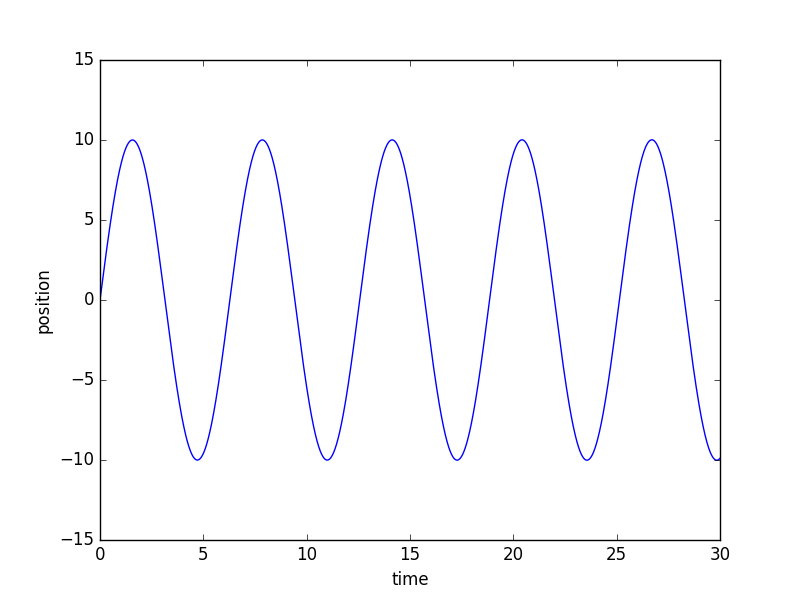
\includegraphics[scale=0.5]{w3fig1.png}
\end{figure}

\begin{figure}[!h]
	\centering
	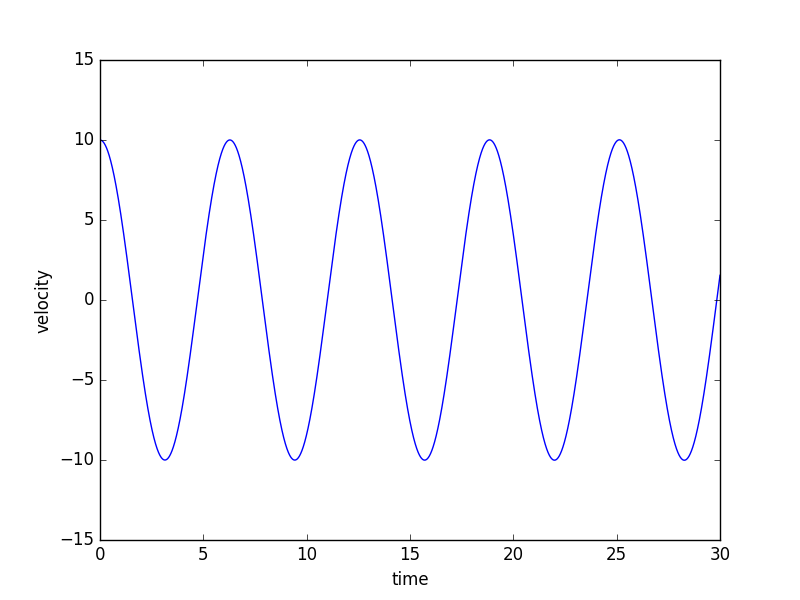
\includegraphics[scale=0.5]{w3fig2.png}
\end{figure}

\newpage

\subsection{}
In the previous problem, we defined $k/m =1$. The equation of motion of the mass on the spring can be solved analytically as the following:\\

$$
m\ddot x = -kx
$$

$$
\ddot x = -x
$$

$$
x = A \cos(t + \phi)
$$

Applying the initial condition we used in the previous problem ($x(0) = 0, \dot x(0) = 10$), the solution becomes

$$
x_{exact} = 10 \sin t 
$$

Applying this solution, we can calculate the global error of the position and the velocity found by using explicit Euler method as a function of time.  \\

\begin{lstlisting}
xexc = 10*np.sin(f[2])
vexc = 10*np.cos(f[2])

plt.figure()
plt.plot(f[2],(xexc-f[0]))
plt.xlabel('time')
plt.ylabel('global error of position')
plt.figure()
plt.plot(f[2],(vexc-f[1]))
plt.xlabel('time')
plt.ylabel('global error of velocity')
plt.show()
\end{lstlisting}

\begin{figure}[!h]
	\centering
	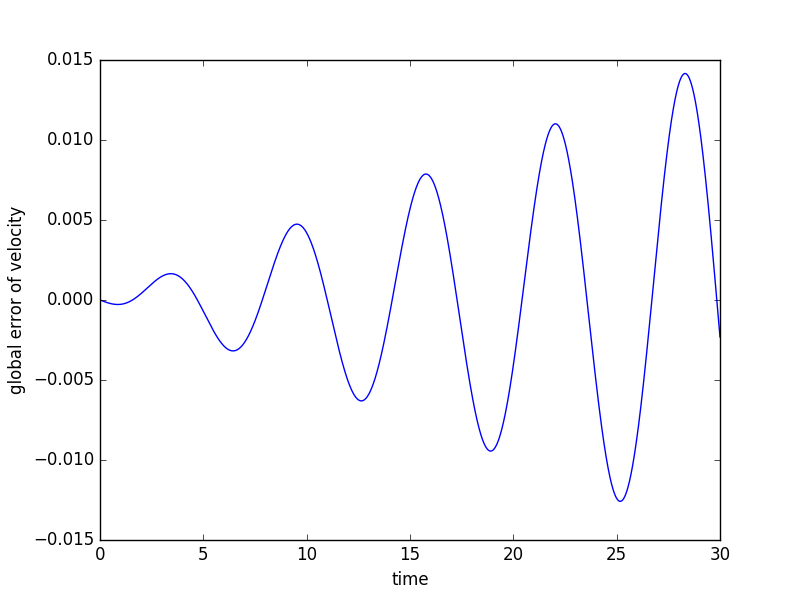
\includegraphics[scale=0.5]{w3fig3.png}
\end{figure}

\begin{figure}[!h]
	\centering
	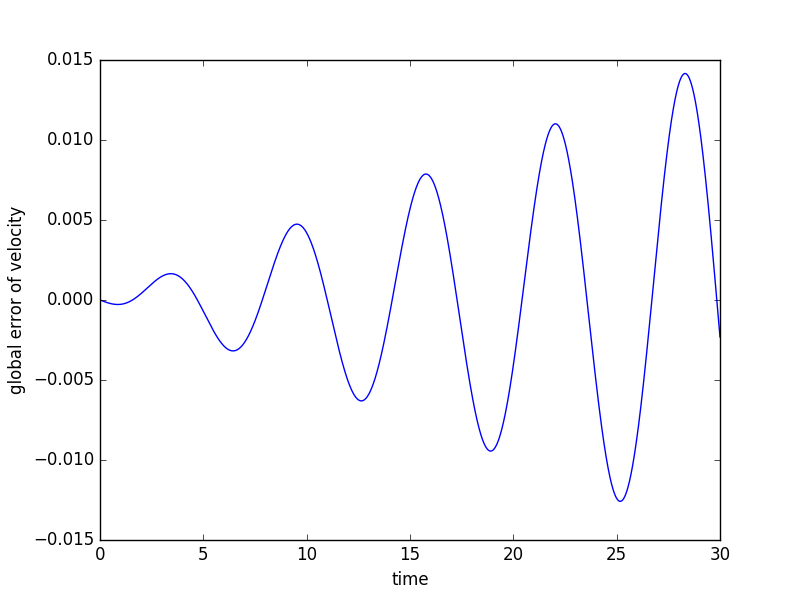
\includegraphics[scale=0.5]{w3fig4.png}
\end{figure}

From the plots of the global error, we see that the error oscillates in the same frequency as the position and the velocity, and the amplitude grows over time from zero. 

\newpage

\subsection{}

I use the same initial condition as the previous problems, and start from $h= 0.0003$. 
\begin{lstlisting}
h0=0.0003
hlist = [h0,h0/2,h0/4,h0/8,h0/16]
xerror = np.zeros(5)
for i in range(5):
    f=spring(0,10,hlist[i],300000*2**i)
    xexc = 10*np.sin(f[2])
    xerror[i] = np.max((xexc-f[0]))
plt.figure()
plt.plot(hlist,xerror,'.')
plt.xlabel('h')
plt.ylabel('truncation error')
plt.show()

\end{lstlisting}

\begin{figure}[!h]
	\centering
	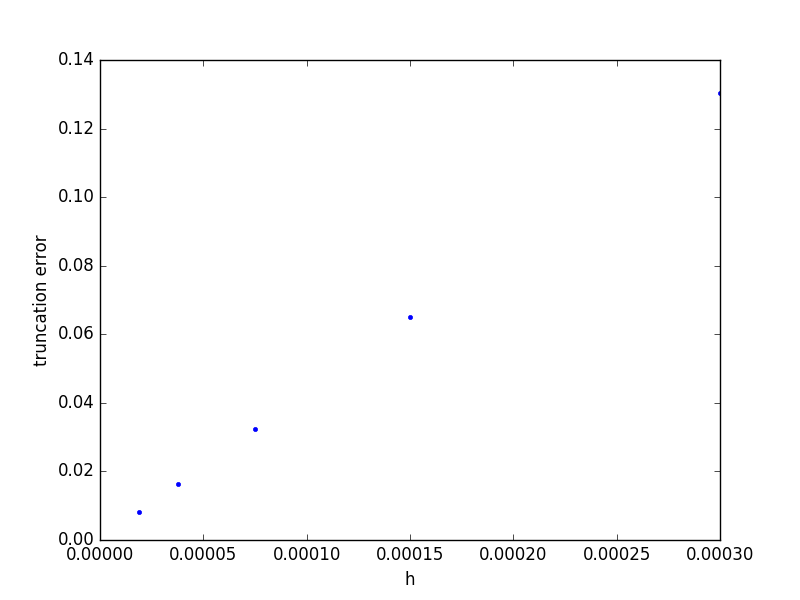
\includegraphics[scale=0.5]{w3fig5.png}
\end{figure}

We can see that the truncation error grows linearly as $h$ increases to 0.0003.\\

\subsection{}
Given the initial condition $x(0)=0, v(0)=10$, the exact solution has a constant energy 100. The code following plots the energy that is calculated by using explicit Euler method from $t=0$ to $t=900$. \\

\begin{lstlisting}
f = spring(0,10,0.0003,300000)
E = np.zeros(np.size(f[2]))
for i in range(np.size(E)):
    E[i] = f[0][i]**2 + f[1][i]**2
plt.figure()
plt.plot(f[2],E)
plt.xlabel('time')
plt.ylabel('energy')
plt.show()
\end{lstlisting}

\begin{figure}[!h]
\centering
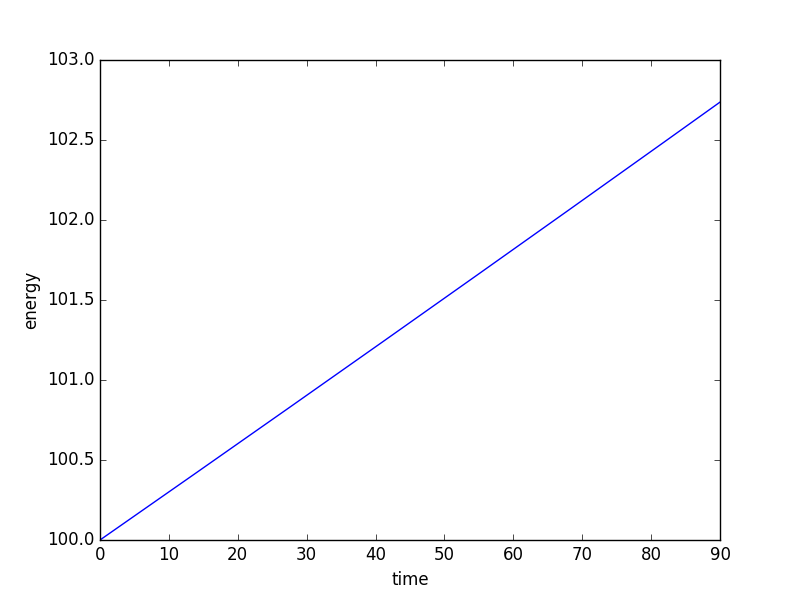
\includegraphics[scale=0.5]{w3fig6.png}
\end{figure}
We can clearly see that the energy deviates from the exact solution linearly over time.\\

\newpage
\subsection{}
In the implicit method, we can express $x_{i+1}$ and $v_{i+1}$ in terms of $x_{i}$ and $v_{i}$ by substituting doing the following algebra.\\

$$
x_{i+1} = x_i + h v_{i+1} = x_i + h (v_{i} - h x_{i+1}) = x_i - h^2 x_{i+1} + hv_i
$$

$$
(1+h^2) x_{i+1} = x_i + hv_i
$$

$$
\therefore x_{i+1} = \frac{x_i} {1+h^2} +\frac{h}{1+h^2} v_i
$$

$$
\therefore v_{i+1} = v_i - hx_{i+1} = v_i - h (\frac{x_i} {1+h^2} +\frac{h}{1+h^2} v_i) = \frac{v_i}{1+h^2} - \frac{h}{1+h^2} x_i
$$

I use the last two equations to update $x$ and $v$ after each time step. I define another function, springimp, that gives series of x, v, and t, computed using the implicit Euler method. \\
\begin{lstlisting}
def springimp(x0,v0,h,n):
    x = np.zeros(n)
    v = np.zeros(n)
    t = np.zeros(n)
    x[0] = x0
    v[0] = v0
    for i in range(n-1):
        x[i+1] = x[i]/(1+h**2)+h*v[i]/(1+h**2)
        v[i+1] = v[i]/(1+h**2)-h*x[i]/(1+h**2)
        t[i+1] = h*(i+1)
    return x,v,t
\end{lstlisting}

First see how the truncation error changes as h changes.\\

\begin{lstlisting}
h0=0.0003
hlist = [h0,h0/2,h0/4,h0/8,h0/16]
xerrorimp = np.zeros(5)
xerror = np.zeros(5)
for i in range(5):
    f=springimp(0,10,hlist[i],300000*2**i)
    g=spring(0,10,hlist[i],300000*2**i)
    xexc = 10*np.sin(f[2])
    xerrorimp[i] = np.max((xexc-f[0]))
    xerror[i] = np.max((xexc - g[0]))
plt.figure()
plt.loglog(hlist,xerrorimp,'r.')
plt.loglog(hlist,xerror,'g.')
plt.xlabel('h')
plt.ylabel('truncation error')
plt.title('Comparing truncation error of Euler implicit & explicit')
plt.show()
\end{lstlisting}

In loglog plots, the truncation error of implicit and explicit Euler methods are almost the same. Both increase linearly as h increases. \\

\begin{figure}[!h]
\centering
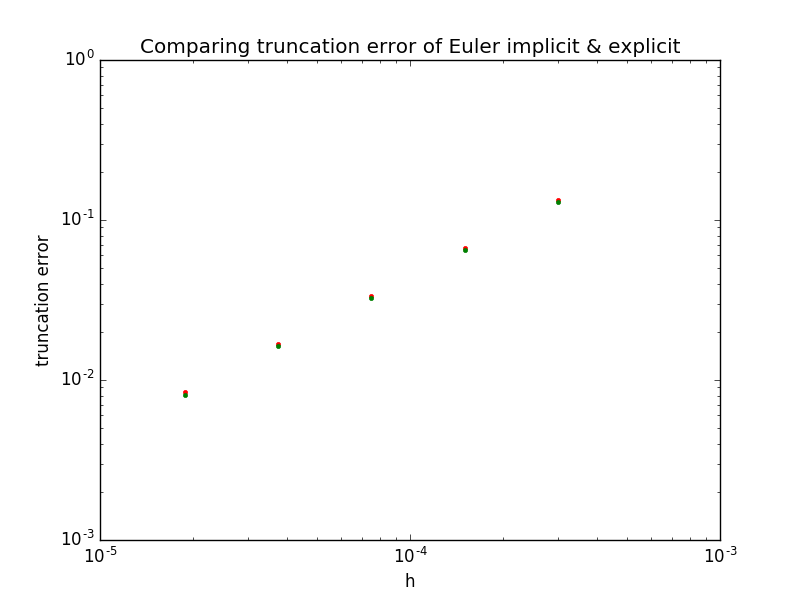
\includegraphics[scale=0.5]{w3fig7.png}
\end{figure}

We can compare how the energy change in implicit and explicit Euler by using the following code.\\
\begin{lstlisting}
f=springimp(0,10,0.0003,300000)
g=spring(0,10,0.0003,300000)
Eimp = np.zeros(np.size(f[2]))
E = np.zeros(np.size(f[2]))
for i in range(np.size(E)):
    Eimp[i] = f[0][i]**2 + f[1][i]**2
    E[i] = g[0][i]**2 + g[1][i]**2
plt.figure()
plt.plot(f[2],Eimp,'r')
plt.plot(f[2],E,'g')
plt.xlabel('time')
plt.ylabel('energy')
plt.show()
\end{lstlisting}

\begin{figure}[!h]
\centering
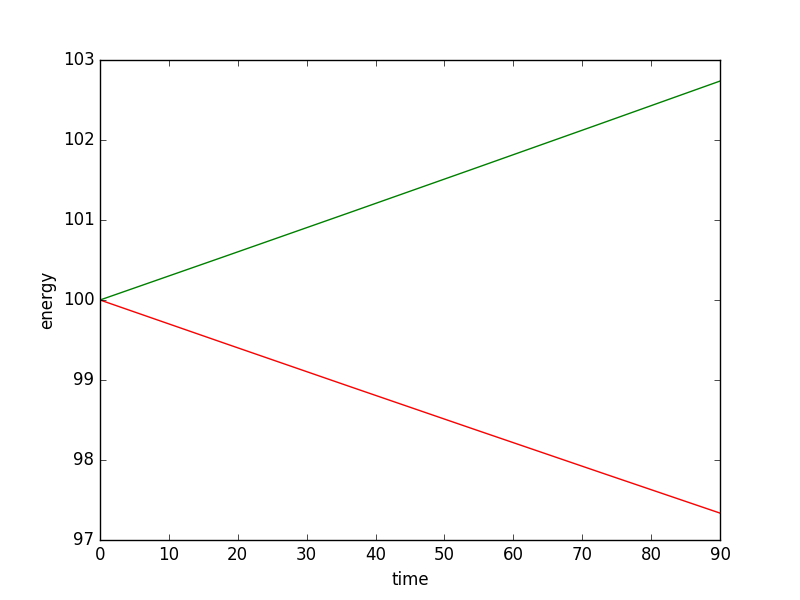
\includegraphics[scale=0.5]{w3fig8.png}
\end{figure}

The plot shows that the energy linearly decreases over time in implicit Euler method, while it increases in the explicit Euler method. As the truncation error plot implies, two plots are symmetric about $E = 100$. In other words, the energy deviates from the exact solution in the same rate for implicit and explicit Euler method.\\
\newpage

\section{Part 2}
\subsection{}
As for the exact solution of a harmonic oscillator, the trajectory in a phase space is a closed circle, since $E^2 = x^2 + v^2$ is a constant, which is a distance from origin in a phase space. From the energy plot of explicit and implicit Euler methods, I can anticipate that the trajectory in phase space will look like a spiral - the trajectory of the explicit Euler method will spiral out, and the implicit will spiral in.\\

\begin{lstlisting}
f=springimp(0,10,0.003,30000)
g=spring(0,10,0.003,30000)
plt.figure()
plt.plot(f[0],f[1],'r')
plt.plot(g[0],g[1],'g')
plt.xlabel('x')
plt.ylabel('v')
plt.show()
\end{lstlisting}
 
\begin{figure}[!h]
\centering
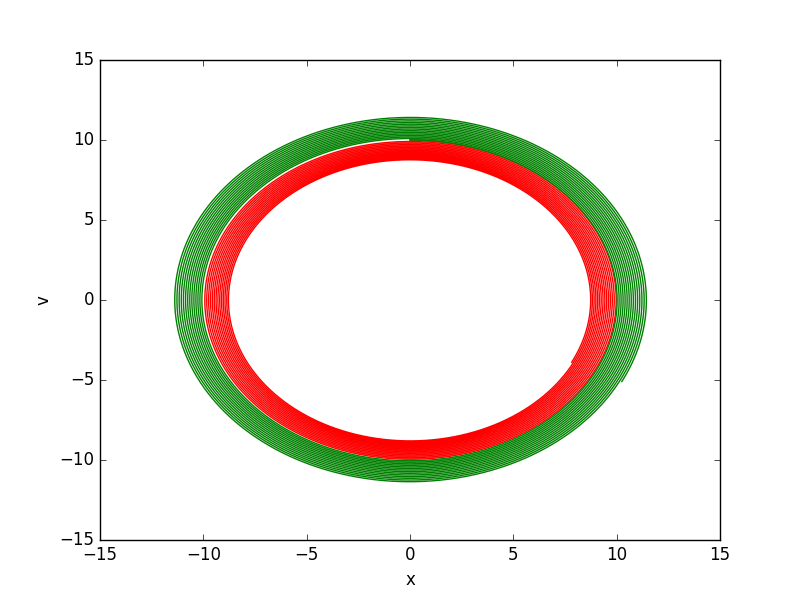
\includegraphics[scale=0.5]{w3fig9.png}
\end{figure}

Indeed we get trajectory spiraling out and in from circle ($x^2 + v^2 = 100$) given the initial condition $x(0)=0, v(0) = 10$. The red (implicit) sprials in, the green (explicit) spirals out. \\

\subsection{}
I define another function springsym for the symplectic method.\\
\begin{lstlisting}
def springsym(x0,v0,h,n):
    x = np.zeros(n)
    v = np.zeros(n)
    t = np.zeros(n)
    x[0] = x0
    v[0] = v0
    for i in range(n-1):
        x[i+1] = x[i]+h*v[i]
        v[i+1] = v[i]-h*x[i+1]
        t[i+1] = h*(i+1)
    return x,v,t
\end{lstlisting}

Plot the trajectory on the top of the phase diagram in the previous problem. I use the same input (initial condition, time steps) as the implicit and explicit Euler methods. \\

\begin{lstlisting}
i = springsym(0,10,0.003,30000)
plt.figure()
plt.plot(f[0],f[1],'r')
plt.plot(g[0],g[1],'g')
plt.plot(i[0],i[1],'b')
plt.xlabel('x')
plt.ylabel('v')
plt.show()
\end{lstlisting}

\begin{figure}[!h]
\centering
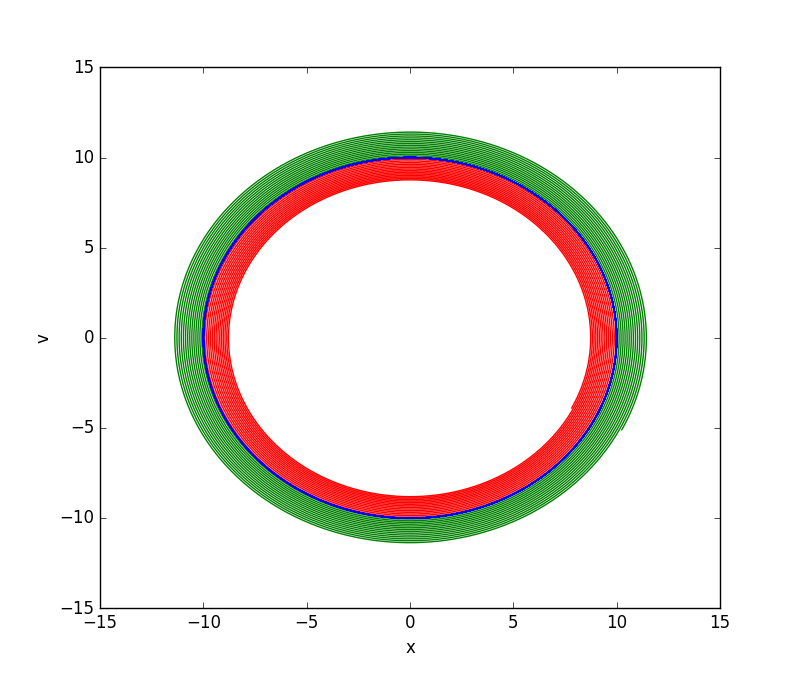
\includegraphics[scale=0.5]{w3fig10.png}
\end{figure}

Clearly, the blue trajectory (symplectic) remains close to the circle, trajectory of the exact solution, even after the same number of revolutions. 

\subsection{}
The energy of the oscillator in the symplectic method looks like a sinusoidal function with a period of $\pi$. \\

\begin{lstlisting}
i = springsym(0,10,0.003,30000)
Esym = np.zeros(np.size(i[2]))
for j in range(np.size(Esym)):
    Esym[j] = i[0][j]**2 + i[1][j]**2
plt.figure()
plt.plot(i[2],Esym,'b')
plt.xlabel('time')
plt.ylabel('energy')
plt.show()
\end{lstlisting}

\begin{figure}[!h]
\centering
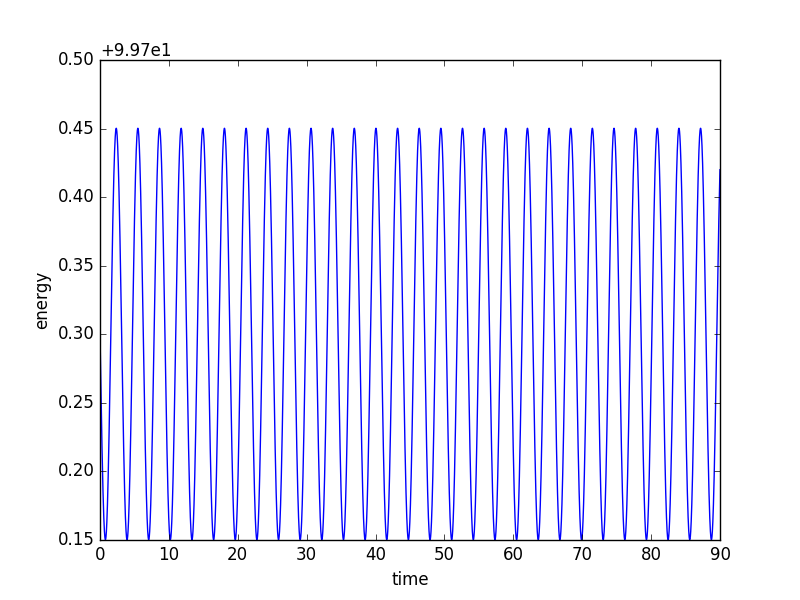
\includegraphics[scale=0.5]{w3fig11.png}
\end{figure}

Compared to the other two Euler methods, the error in energy does not grow but only oscillates. (red : implicit, green : explicit, blue : symplectic)\\

\begin{figure}[!h]
\centering
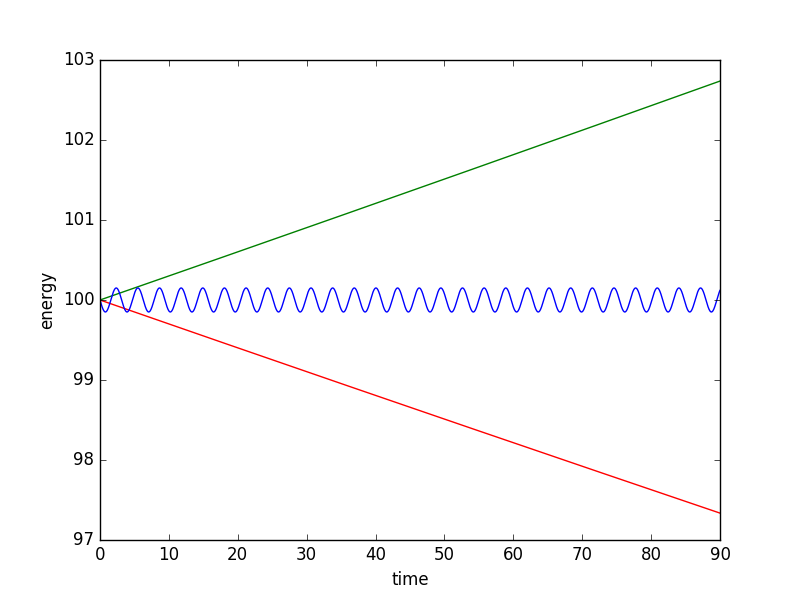
\includegraphics[scale=0.5]{w3fig12.png}
\end{figure}

\newpage

\subsection{}
The red is a position according to the symplectic method and the green shows the exact solution. At $t=9000$, the position estimated by symplectic method is lagging by around $0.3$. Thus, the rate of lagging is about $3 \times 10^{-5}$ period per cycle. 
\begin{figure}[!h]
\centering
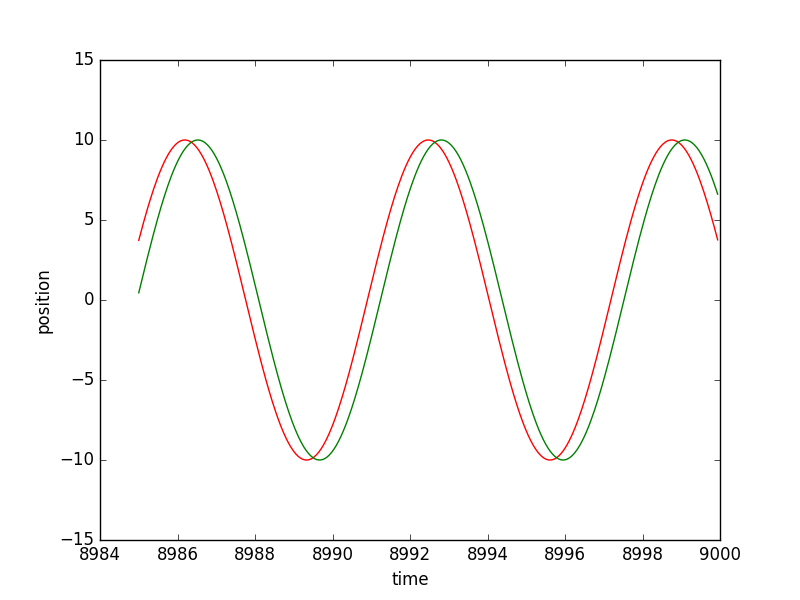
\includegraphics[scale=0.5]{w3fig14.png}
\end{figure}

\section{Correction}
With higher $h$ we see that the energy in implicit and explicit Euler methods do not deviate linearly.\\
I increased $h$ by 10 times. The red line is implicit Euler, green is explicit. Note that the curves are not symmetric in a linear plot: the energy converges to 0 for implicit method, and diverges to infinity faster and faster for explicit method. However in loglog plot, the energy plots are symmetric because they increase/decrease in the same power.\\

\begin{figure}[!h]
\centering
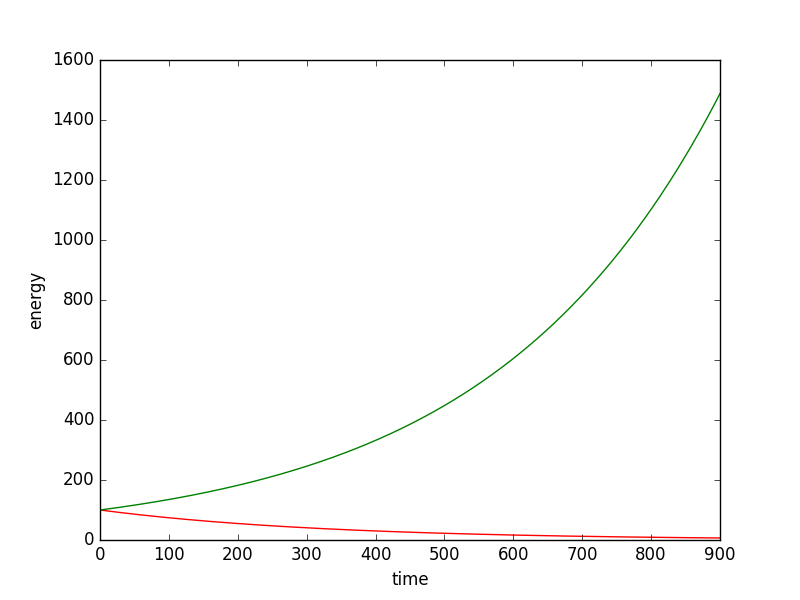
\includegraphics[scale=0.5]{w3fig15.png}
\end{figure}

\begin{figure}[!h]
\centering
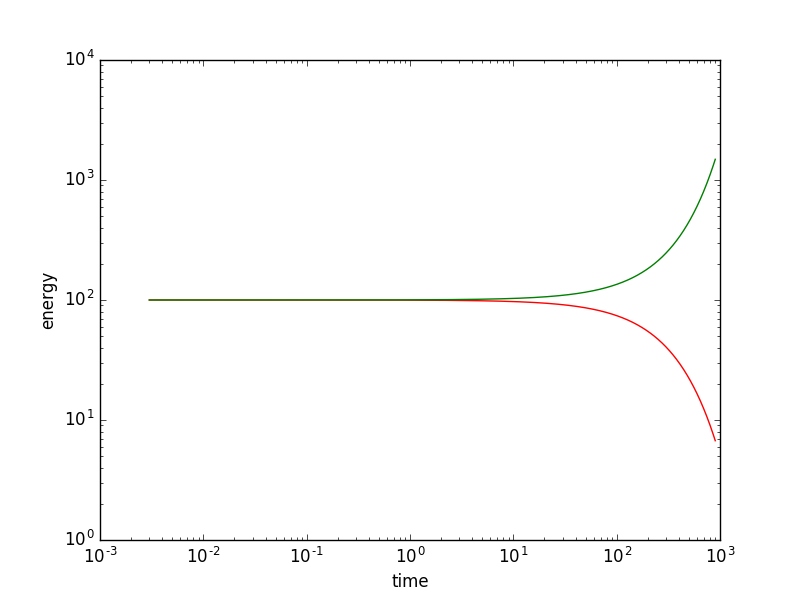
\includegraphics[scale=0.5]{w3fig17.png}
\end{figure}
\newpage
Also with a larger $h$, the solution of the symplectic method will noticeably deviate from the analytical solution. The red line corresponds to the symplectic method, and the blue line is an exact solution. Note that the red deviates in a periodic manner, and the angular frequency is $\pi$ just like what we saw in 2.3.\\
\begin{figure}[!h]
\centering
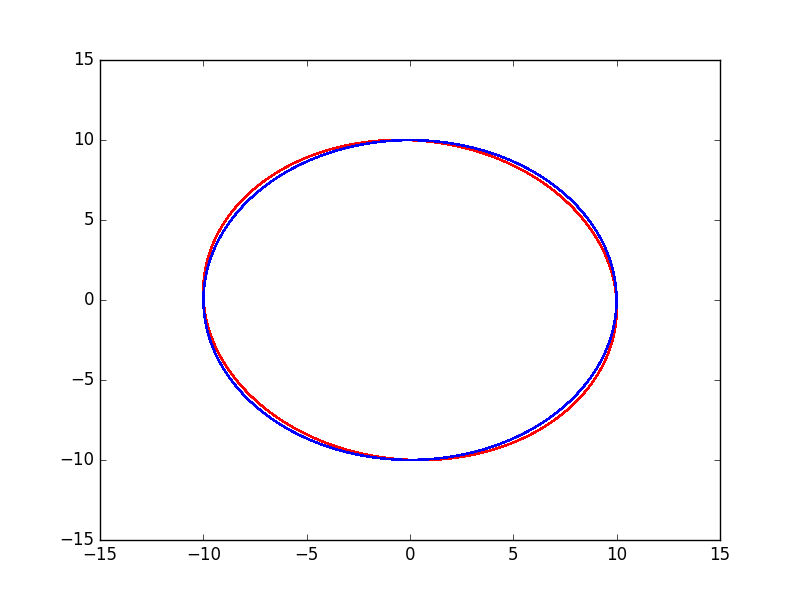
\includegraphics[scale=0.5]{w3fig16.png}
\end{figure}


\end{document}
